\documentclass[a4paper, 12pt]{article}
%\documentclass[a4paper, 12pt, draft]{article} % don't include images, leave a border of same size...great

% Variable de compilation
\newif\ifbeamer
\beamerfalse
\newcommand{\beamer}[2]{\ifbeamer #1 \else #2 \fi}
%%%

%\usepackage[latin1]{inputenc}
\usepackage[utf8]{inputenc} % manage utf8 encodage 
%\usepackage[english]{babel} % for french document ! dirty enumerate style,+ bad change rectangle colors for section linking.
\usepackage{fancyhdr} % for heading
\usepackage{listings}
\usepackage[colorlinks=true, urlcolor=blue]{hyperref} % url, link
\usepackage{graphicx}
\usepackage{geometry}

%\usepackage[cmex10]{amsmath, mathtools}
\usepackage{amsmath,amssymb,amsbsy,amsfonts,amsthm}
\usepackage{multirow}
\usepackage{bm}
\usepackage{enumerate}
\usepackage{url}
\usepackage[ruled,vlined]{algorithm2e}
\usepackage{fancyvrb}
\usepackage{yfonts}

\usepackage{wrapfig}
\usepackage{tikz}
    %\input{../tikz.conf}
    
\usetikzlibrary{bayesnet}
    
%%%%%%%%%%% Box 
\usepackage{calc}%    For the \widthof macro
\usepackage{xparse}%  For \NewDocumentCommand
\newcommand{\tikzmark}[1]{\tikz[overlay,remember picture] \node (#1) {};}

%%%%%%%%%% Math
\renewcommand{\text}{\textnormal}
\newcommand{\pr}{\mathbf{p}}
\newcommand{\E}{\mathbb{E}}
\newcommand{\divkk}{\mathbb{K}}
\newcommand{\entropy}{\mathbb{H}}
\newcommand{\gem}{\mathrm{GEM}}
\newcommand{\Mult}{\mathrm{Mult}}
\newcommand{\DP}{\mathrm{DP}}
\newcommand{\IBP}{\mathrm{IBP}}
\newcommand{\M}{\mathcal{M}}
\newcommand{\V}{\mathcal{V}}
\newcommand{\N}{\mathcal{N}}
    
\makeatletter
\NewDocumentCommand{\DrawBox}{s O{}}{%
    \tikz[overlay,remember picture]{
    	\IfBooleanTF{#1}{%
    		\coordinate (RightPoint) at ($(left |- right)+(\linewidth-\labelsep-\labelwidth,0.0)$);
    	}{%
    	\coordinate (RightPoint) at (right.east);
    }%
    \draw[red,#2]
    ($(left)+(-0.2em,0.9em)$) rectangle
    ($(RightPoint)+(0.2em,-0.3em)$);}
}

\NewDocumentCommand{\DrawBoxWide}{s O{}}{%
	\tikz[overlay,remember picture]{
		\IfBooleanTF{#1}{%
			\coordinate (RightPoint) at ($(left |- right)+(\linewidth-\labelsep-\labelwidth,0.0)$);
		}{%
		\coordinate (RightPoint) at (right.east);
	}%
	\draw[red,#2]
	($(left)+(-\labelwidth,0.9em)$) rectangle
	($(RightPoint)+(0.2em,-0.3em)$);}
}
\makeatother
%%%%% ! Box

\geometry{
      a4paper,
	    body={160mm,260mm},
	    left=25mm,top=20mm,
	    headheight=4mm,headsep=8mm,
        footskip=10mm,
        }
                                              

%%%%%%%%%%%%%%%%%%%%%%%%%%%%%%%%%%%%%%%%%%%%%%%%%%%%%%%%%%%%%%%%%%%%%%%%%%%%%%%%%%%%%%%%%%%%%%%%%%%%%%
%%%%% => Internal
%%%%%%%%%%%%%%%%%%%%%%%%%%%%%%%%%%%%%%%%%%%%%%%%%%%%%%%%%%%%%%%%%%%%%%%%%%%%%%%%%%%%%%%%%%%%%%%%%%%%%%

% itemize item def
%% \begin{itemize}\itemsep2pt % example space betwew item
%\renewcommand{\FrenchLabelItem}{\textbullet}
\renewcommand{\labelitemi}{$\bullet$}
\renewcommand{\labelitemii}{$\cdot$}
\renewcommand{\labelitemiii}{$\diamond$}
\renewcommand{\labelitemiv}{$\ast$}

% equation reference
\renewcommand{\theequation}{\thesection.\arabic{equation}}

%%%%%%%%%%%%%%%%%%%%%%%%%%%%%%%%%%%%%%%%%%%%%%%%%%%%%%%%%%%%%%%%%%%%%%%%%%%%%%%%%%%%%%%%%%%%%%%%%%%%%%
%%%%% => Alias
%%%%%%%%%%%%%%%%%%%%%%%%%%%%%%%%%%%%%%%%%%%%%%%%%%%%%%%%%%%%%%%%%%%%%%%%%%%%%%%%%%%%%%%%%%%%%%%%%%%%%%

% write code
\lstnewenvironment{C}[1]
{\lstset{language=C,
      frame=tBRl,
      basicstyle=\scriptsize,stringstyle=\emph,showstringspaces=false,
      numbers=left,numberstyle=\tiny,
      breaklines=true, columns=flexible, title={#1}}
}{}
      
%%%%%%%%%%%%%%%%%%%%%%%%%%%%%%%%%%%%%%%%%%%%%%%%%%%%%%%%%%%%%%%%%%%%%%%%%%%%%%%%%%%%%%%%%%%%%%%%%%%%%%
%%%%% => Preambles Pages
%%%%%%%%%%%%%%%%%%%%%%%%%%%%%%%%%%%%%%%%%%%%%%%%%%%%%%%%%%%%%%%%%%%%%%%%%%%%%%%%%%%%%%%%%%%%%%%%%%%%%%

\pagestyle{fancy}
\fancyhf{} % remove default headers
\fancyfoot[C]{\thepage}
\renewcommand{\footrulewidth}{0.3pt}
\renewcommand{\headrulewidth}{0.3pt}


%\author{Adrien Dulac}

\title{
      %\vspace{2cm}
      \Large{Social Networks Properties Through Mixed Membership Models}\\
            --\\ }

%\date{avril 2015}

\newtheorem{definition}{Definition}[section]
\newtheorem{proposition}{Proposition}[section]
\newtheorem{theorem}{Theorem}[section]

\begin{document}
\fancypagestyle{plain}{
      \fancyhf{}
      %\fancyhead[L]{\includegraphics[scale=0.4]{ipb.eps}}
      \renewcommand{\footrulewidth}{0pt}
      \renewcommand{\headrulewidth}{0pt}
}
\maketitle


\textbf{Keywords}: Burstiness, preferential attachment, Assortativity, community detection, link prediction, dyadic relation, latent class model, latent feature model. Matrix Factorization, Bayesian, uncertanty, regularisation

\section{Introduction}

We provide formal definitions of fundamental properties of social networks which are consistent within the probabilistic framework. We study those properties on two general models based on Bayesian nonparametric prior namely the Hierarchical Dirichlet Process (HDB) and the Indian Buffet Process (IBP). We show the relation between those properties and the models and how they can be captured in a learning problem. Additionally, we propose an adaptation of priors which gives a better interpretation of models in terms of assumptions on social networks and lead to better prediction performance.


\section{Motivations}
Recently, several complex Bayesian models based on latent variables to explain the structure of social networks have been introduced [mmsb, ilfrm, etc]. This work was mainly evaluated on prediction tasks, such as link prediction or communities detection. However, few works have been done concerning the study of the intrinsic capacity of the models to model basic properties that arise in social networks, such as the dynamics of degree distribution known to exhibit the preferential attachment effect [barabasi, web..] or the homophily effect[ref].
% For exemple, the heavily study Latent Dirichlet Allocation Model LDA model, being a particular of Mixed Membership Stochastic Blockmodel (MMSB) for networks, made no epistomological claim about the conjugacy used. In this work we found that conjugacy played a role in the ability of the model to capture some properties.
~\\


(++ Indeed the most heavily studied properties in network was the degree distribution and the mixing pattern (homophily/assortativity) tableaux !)

(++ not clear consensus of the formalism of properties and measure evaluation not clear consensus, and whatsoever for the homophily propertie the feature the definition are usually for single attribute... We consider a general vector . (and latent in our approach )

(++ Probabilistic models we are interested in provide two ways of representing the data or network. One fall in the paradigm of mixture models and the other in the latent feature modeling. A motivation of those two modeling paradigm is that they are consistent with two key nonparametric prior for discrete data, namely the Dirichlet process (DP) and the the Indian Buffet Process (IBP). Many baysian model can be view as equivalent to truncated models with nonparametric priors. This provide a motivation to study those models)

(++ We will consider two hierarchical baysian model for relational learning. It appears that those model can be derive either with Hierachical Dirichlet Process (HDP) and Beta Process (BP). Those two constitute priors that lead to posterior distribtution that account for burstiness in latent features. But are they able to handle burstiness at the degree level ?)


In the next section we will, first, explain the mathematical background in a machine learning context. Then, we will review the formal definition of properties of interest in social networks, and how this is translated in terms of assumptions within Bayesian priors. Secondly, we will study how those properties can be satisfied within our Bayesian framework. Finally, we will show empirical results (on synthetic and real datasets) to support our claims.~\\

In the following paper we focus on the following properties: (move this elsewhere ?)
\begin{itemize}
	\item Burstiness / Preferential Attachment (relation between them ?)
	\item Local Preferential Attachment (inside communities)
		\begin{itemize}
			\item The nodes degree follow a power law...
			\item The first derivative of the degree distribution is positive...
			\item The probability to observe a link for a node increase with its degree.
			%One way to show a distribution is bursty is to show that the second derivative of the survival function is strictly positive.
			% La burtsiness est aussi appelé variation régulière en statistique.
		\end{itemize}

	\item Homophily
		\begin{itemize}
			\item The probability to have a link between two nodes increases if their similarity increase.
		\end{itemize}
\end{itemize}

\paragraph{Questions: Formal definitions ?}~\\
We need to settle the right formal definition of properties, and find a consensus with the graph mining community (voir aussi dicussion au/et section suivante)


%Study the poisson binomial distribution for the out links of a node. This is the degree distribution and should be bursty to have commmunity in networks.

\section{Related Work}
= Prop
Burstiness on topic model:
Modeling Word Burstiness Using the Dirichlet Distribution (DCM)
Accounting for Burstiness in Topic Models (DCMLDA)
LDA bursty on topics
Proposal of a-MMSB in : Scalable Inference of Overlapping Communities
with high diagonal only...

to read: Stochastic blockmodels and community structure in networks

= Model
Recent work on MMSB and copula: Copula Mixed-Membership Stochastic Blockmodel with Subgr
oup Correlation


\section{Background}
Relational learning provides a framework for predictive task in graph based data.  Even though we focus on  graphical models we seek for a general representation of our models. "Identify role of latent variables and potential seed for networks fundamental property". A natural frameworks that arise from latent factorization perspective allows us to emphasize core structural similarities. (paragraph in progess...)

In order to model this parameter we pursue two concurrent modeling approaches, but still within a Bayesian frameworks.

\paragraph{}
The first model we focus on falls down in the \emph{latent class} category. In this link prediction model, each node has a latent feature vector of class proportion. For each single interaction between two nodes, one class is draw for each one. The probability to have a link is only conditioned on the classes assignment. This model has a direct interpretation in term of blockmodel [ref], by predicting the link structure according to which blockmodel nodes belong to. Our reference for the class based model is the Mixed Membership Stochastic Blockmodel (MMSB) ~\cite{MMSB} and its nonparametric version using a Hierarchical Dirichlet Process prior (HDP)~\cite{HDP}.

(-- Change the latent feature model to the Mixed Membership Deterministic Blockmodel (MMDB) vs MMSB. (see graphical model.)

\paragraph{}
The second model of interest is related to the \emph{latent feature} category. Here, each node has an associated feature vector and the model uses the features to predict the link structure. This approach has an interpretation in terms of homophily in network. Our reference for the feature based model is a binary matrix factorization  (BMF)~\cite{BMF} and its nonparametric version using a Indian Buffet process (IBP)~\cite{IBP} known as the Infinite Latent Feature Model (ILFM)~\cite{ILFRM}.

\paragraph{}
The difference between the two approaches can be expressed by the structure of the Bayesian network or Graphical Model (GM) behind the generative model, and the form of the prior choose for the random variables distribution \ref{fig:bayes_net}. Nevertheless the GM formalizes the regularization applied when fitting the model, but both models can have a common interpretation in terms of matrix factorization. Thus, pursuing the approach in~\cite{DCA}, it allows us to highlight a structural similarity in the general field of relational learning. (pas clair ?)

\paragraph{}
Without loss of generality, we focus on social networks with binary relationships. Our object of interest is the topology of the network representing the presence or absence of links between nodes in the graph. The network can be either directed or not. For a network with $N$ nodes, we represent the topology by an adjacency matrix $Y \in \{0,1\}^{N\times N}$ associated to a graph $G = (V,E)$, where $V$ is a set of nodes representing entities, $E \in V \times V$ is a set of edges representing relationships between pairs of entities. From a probabilistic point of view, the network topology is modeled using a kernel with a Bernoulli density. The parameters of the Bernoulli is the probability to observe a link between two nodes.

\paragraph{(mettre en avant le sens des deux modeles)}
We define a matrix of weight interactions $\Phi \in W^{K\times K}$ with $W$ the space of weights, where $K$ is the number of classes or features. Let $\Theta \in \mathcal{F}^{N\times K}$, be a matrix where each row $i$ represents the latent feature vector associated to the node $i$,  and $\cal{F}$ the latent feature space. For the latent class model, this feature vector represents the proportion of classes the node belongs to. In this framework the network is generated with the following density:
\begin{equation}
    Y \sim \mathrm{Bern}(\sigma(\Theta \Phi  \Theta^T))
\end{equation}
where $\sigma$ is a function that map values to a probability space. When $\sigma$ is the identity function, the expectation of the observation takes a matrix factorization (bilinear) form, and is related to Discrete Component Analysis (DCA)~\cite{DCA}:
\begin{equation}
E_{y \sim p(y|\Theta, \Phi)}[Y] = \Theta \Phi  \Theta^T
\end{equation}

This matrix factorization approach of the Bayesian model is in due to the likelihood of the model when applying the sum rule over the latent variables. Indeed the probability to have a link for the interaction $(i,j)$ is:
\begin{equation}
\pr(y_{ij}=1 \mid \Theta, \Phi ) = \sum_{k, k'} \pr(y_{ij}=1\mid\phi_{k,k'}) \pr(k \mid\theta_i) \pr(k' \mid \theta_j)
\end{equation}


The questions that arise are:
\begin{itemize}
	\item What kind of properties the model can capture or learn on networks ?
	\item Which constraint on the models can come with an consistent interpretation of latent variable along with the concepts of communities structure and homophily in social networks  ?
\end{itemize} 

In the next session we review the models of interest.

\section{Homophily}
\hspace{2em} \emph{Birds of a feather flock together} ~\\

%\paragraph{Formal Definition}~\\

Homophily describes the fact that two nodes are more likely to be connected if they share common characteristics~\cite{mcpherson2001birds,lazarsfeld1954friendship}. So, the more similar the nodes, the more likely is it to be connected. In their research on dynamic attributed networks where the attributes are discrete (e.g. age, gender etc.).Some definition has been proposed~\cite{la2010randomization}, but they consider unimodal feature and lack of generality to use them in a Bayesian framework. We proposed a more general definition of homophily at the model level:

\begin{definition}[Homophily]
	Given  a model parameters and a function $ \M=\{\Theta, \Phi, s\}$, accounting respectively for latent features, weight interactions, and a similarity function $s(. ;\Theta, \Phi)$ defined on $V\times V$ and parametrized by the model parameters, we consider that the model exhibits homophily if:
	\begin{align*}
	&\text{if }  s(i,j) > s(i',j') \text{ then } \E_\Phi[\pr(y_{ij}=1 \mid \Theta)] > \E_\Phi[\pr(y_{i'j'}=1  \mid \Theta)] \\
	&\forall (i,j,i',j') \in V^4 \nonumber 
	\end{align*}
In this case we way that the model is homophilic.
\end{definition}

The similarity aims at measuring the closeness between two node, given the (latent) features. The homophily evaluate if the order is preserved between the similarity and the probability to create a link between two node when averaging on the weight matrix of the model.

In both models, we can assess a natural similarity which arises from the Bernoulli parameter. That is to say that the probability to have a link for the couple $(i,j)$ is defined as the bilinear form such as: 
\begin{equation}
s(i,j) = \theta_i \Phi \theta_j^\top
\end{equation}

\begin{proposition}[]
Let's suppose a model $ \M=\{\Theta, \Phi, s\}$ with the similarity measure defined as $s(i,j) = \theta_i \Phi \theta_j^\top$, the ILFM and MMSB models are homophilic.
\end{proposition}
\paragraph{Proof} 
Suppose that for two couple of nodes $(i,j,i',j') \in V^4$ we have $s(i,j) > s(i',j')$ with $s(i,j) =\theta_i \Phi \theta_j^\top$, and $\sigma$ a either strictly increasing function or the identity function. We have:
\begin{align}
obj &=\E_\Phi[\pr(y_{ij}=1 \mid \Theta)] - \E_\Phi[\pr(y_{i'j'} = 1  \mid \Theta)] \\
&= \int_{\Phi} \pr(y_{ij}=1 \mid \Theta, \Phi ) \pr(\Phi) d\Phi - \int_{\Phi}\pr(y_{i'j'}=1 \mid \Theta, \Phi ) \pr(\Phi) d\Phi \\
&= \int_\Phi ( \pr(y_{ij}=1 \mid \Theta, \Phi )  - \pr(y_{i'j'}=1 \mid \Theta, \Phi ) )\pr(\Phi) d\Phi \\
&=  \int_\Phi ( \sigma(\theta_i \Phi  \theta_j^T) -\sigma(\theta_{i'} \Phi  \theta_{j'}^T) )\pr(\Phi) d\Phi
\end{align}
Since $\sigma$ are strictly increasing (or the identity), the left hand part and the right hand are strictly positive function we have $\E_\Phi[\pr(y_{ij}=1 \mid \Theta)] > \E_\Phi[\pr(y_{i'j'} = 1  \mid \Theta)]$.~\\


In this case, the homophily effect holds in both models as it is the parameter of the Bernoulli. In other words, it is the probability to observe a link between $i$ and $j$. Thus the metric for the network topology and the node similarity are the same. Nevertheless it is not obvious to state the role that plays latent variables for the homophily because of the weak constraints applied on the interactions matrix $\Phi$. In other word we loose the intuition behind the similarity. ~\\

But It is important to note that the metric for the topology of the network and the node similarity has not to be same, as it is a very restrictive assumption. Especially for an real networks, node features may be accessible and without a priori knowledge a natural metric that can be applied on both real network with real features and the model with latent features is cosinus based measure.~\\

A natural constraint for the \emph{similarity metric} is to use some cosinus based measure. Furthermore those measure only rely on the latent/real feature of nodes. It thus make them applicable to model and real networks. We will consider next the dot product as our similarity based measure; $s(i,j) = \theta_i \theta_j^\top$.~\\

A natural constraint for the \emph{topology metric}, would be to stay consistent with the notion of communities in networks. In this case nodes belonging to the same community would be more likely to be linked. One way to encode this believe is to have strong values in the diagonal for the interaction matrix $\Phi$. Moreover by defining decreasing weights from the diagonal, we allow inter-communities links and define a hierarchies (ie an order) between the possible interactions between the communities. We develop this idea with two adapted prior for each models. A matrix normal prior for the ILFRM model and a matrix beta for the MMSB model.~\\


\begin{proposition}[] \label{prop:hom_mn}
Let's suppose a model $ \M=\{\Theta, \Phi, s\}$ with the similarity measure defined as $s(i,j) = \theta_i \theta_j^\top$ and $\sigma$ a strictly increasing function or the identity. Let's suppose a $K\times K$ matrix normal prior over weight matrix such as $\Phi \sim \N_K(M, U, V)$ and the mean matrix $M$ be a diagonal matrix. Then homophily hold for $\M$ if $M=\Lambda I_K$ with $\Lambda > 0$.
\end{proposition}
\paragraph{Proof} 
Suppose that for two couple of nodes $(i,j,i',j') \in V^4$ we have $s(i,j) > s(i',j')$, with $s(i,j) =\theta_i \theta_j^\top$. We first examine the difference of expectations:

\begin{align}
&\E_{\Phi}[\pr(y_{ij}=1\mid \Theta)] - \E_{\Phi}[\pr(y_{i'j'}=1\mid \Theta)] =  \E_{\Phi}[\sigma(\theta_i \Phi \theta_j)] -  \E_{\Phi}[\sigma(\theta_{i'} \Phi \theta_{j'})] \\
&= \E_{\Phi}[\sigma(\theta_i \Phi \theta_j) - \sigma(\theta_{i'} \Phi \theta_{j'})]
\end{align}
Because $\sigma$ is stricly increasing (or the identity), we have the following equivalence:
\begin{equation}
\E_{\Phi}[\sigma(\theta_i \Phi \theta_j) - \sigma(\theta_{i'} \Phi \theta_{j'})] > 0  \iff \E_{\Phi}[\theta_i \Phi \theta_j - \theta_{i'} \Phi \theta_{j'}] > 0 
\end{equation}
Then according to matrix normal property we have:
\begin{align}
\E_{\Phi}[\theta_i \Phi \theta_j] &= \E_{\Phi}[\N_K(\theta_iM\theta_j, \theta_iU\theta_i, \theta_jV\theta_j)] \\
&= \theta_iM\theta_j \\
&= \Lambda \theta_i \theta_j
\end{align}
It follows that:  
\begin{equation}
\E_{\Phi}[\theta_i \Phi \theta_j] - \E_{\Phi}[\theta_{i'} \Phi \theta_{j'})] > \Lambda (\theta_i \theta_j - \theta_{i'} \theta_{j'} )
\end{equation}
Homophily is satisfied for $\Lambda > 0$.

~\\

Proposition \ref{prop:hom_mn} highlight a generalization of the MMSB model where the correlation between class are correlated to their proximity. This enable the interpretation of class as communities because node who belongs to the same class have a higher probability to binds. Note that this generalization conserve the conjugacy property of the model and therefore his efficient implementation.


\section{Burstiness}
\hspace{2em} \emph{The rich get richer and the poor get poorer} ~\\

%\paragraph{Formal Definition}~\\

The preferential attachment states that a node is more likely to create connections with nodes having a high degree. To take into account this behavior, in the BarabasiAlbert (BA) model, each node is connected to an existing node with a probability proportional to the number of links of the chosen node. This leads to scale-free networks, characterized by a degree distribution with a heavy tail which can be approximated by a power law distribution such that the fraction of nodes $\pr(d)$ having a degree $d$ follows $\pr(d) \sim d^{-\gamma}$ where $\gamma$ ranges typically between 2 and 3~\cite{barabasi1999emergence}. An equivalent notion is the burstiness, studied by~\cite{church1995poisson}, which conveys the same idea : rich get richer or the more you have, the more you will get. In~\cite{clinchant2008bnb}, a formalized definition has been proposed. According to the authors:

\begin{definition}[Burstiness]
	A discrete distribution $\pr$ is bursty if and only if for all integers $(n, n')$, $n \geq n'$ :
	
	\begin{equation}
	\pr(d \geq n'+1 \mid d \geq n') > \pr(d \geq n+1 \mid d \geq n) 
	\end{equation}
	 A distribution which verifies this condition is said to be bursty.
\end{definition}

In~\cite{clinchant2010information}, this definition has been generalized to the continuous case but, in the sequel, we will retain this first definition since we focus on discrete distributions.~\\

The burstiness can appear for different various variable in a model. In this paper we consider three different schemes at the node and feature level, that constitute some basic assumptions on networks:

\begin{proposition}~\\
for all $i,j \in V^2$ and $k \in \{1,.., K\}$, we have:
\begin{itemize}
	\item Preferential Attachment: the distribution of degree $d_i$ is bursty iff $f_i$ is a stricly increasing function of n with: $$f_i(n)=\pr(y_{ij}=1 \mid d_i=n)$$
	\item Local Preferential Attachment: Given a class $c \in \{1,..,K\}$, and a degree restricted to nodes who belongs to this class $d_{ic}$, the distribution of degree $d_{ic}$ is bursty iff $f_{i,c}$ is a stricly increasing function of n with: $$f_{i,c}(n)=\pr(y_{ij}=1 \mid d_i=n, c)$$
	\item Feature burstiness (block/class burstiness ?:s): the distribution over the number of membership of each class is bursty iff  $f_k$  is a stricly increasing function of n with: $$f_k(n) = \pr(\theta_{ik} \mid \theta_{\bm{.}k}^{-ik}=n)$$ 
\end{itemize}
\end{proposition}

We justify this approach in the supplementary materials~\ref{burst_proof}. One can see that the approach makes the link with the classical definition of preferential attachment. Furthermore one can see that the similaraty between th functions we track $(f_i, f_{i,c}, f_k)$ and the typical Gibbs updates. The difference is that we want to assess the generative model given the data and parameters of the model (ie the model has converged). Hence we are looking if the topological property of burstiness can be handle by the model once it learned from the data.~\\


%Considering the nodes projection on latent variables, the projections for the nodes we evaluate might be considered either known or not known ($\Theta$ or $\Theta^{-ij}$) depending on the case study of preferential attachment or local preferential attachment.~\\

\section{Models}
 \hspace{2em} \emph{Yet another view} ~\\
\label{fig:bayes_net}

Our two models use prior distributions that fall into the two major classes of discrete nonparametric priors. The Hierarchical Dirichlet Process (HDP) that generalizes the Dirichlet-Multinomial compound distribution for infinite mixtures models. On the other hand, the Indian Buffet Process (IBP), which is the generalization of the Beta-Bernoulli compound distribution, generates infinite binary matrices.The nonparametric models in their finite version are equivalent to well-known models such as Latent Dirichlet Allocation, widely used for text analysis, and Mixed Membership Stochastic Blockmodel which is an adaptation for relational learning.~\\


We adopt the following notation; if a matrix has a negative index superscript, it indicates that the values corresponding to this index are excluded. A dot $\bm{.}$ in the index means that we marginalize over all possible values.


\subsection{Latent Feature}
In the latent feature models, the features are distributed according to an Indian Buffet Process (IBP), and the weights interaction according to a Gaussian :
\begin{align}
\Theta &\sim \IBP(\alpha)  \quad\text{ is a } N\times K \text{ matrix}\\
\phi_{mn} &\sim N(0, \sigma_w) \quad\text{ for } m,n \in \{1, .., K\}^2
\end{align}
The observation level is defined by deterministically selecting the row of $\Theta$ that encodes the latent features for each nodes that interact. Hence for a node $i$, we note his feature vector by $F_i = \theta_i$ and for $i, j \in V$ we have:

\begin{align}
y_{ij} &\sim \mathrm{Bern}(\sigma(F_i \Phi F_j^\top))
\end{align}
Finally the function $\sigma(x)= \frac{1}{1 + e^{-x}}$ is the sigmoid function to map $[-\infty, +\infty]$ values to [0,1].

\begin{figure}[h]
	\centering
	\minipage{0.4\textwidth}
	\scalebox{0.9}{
	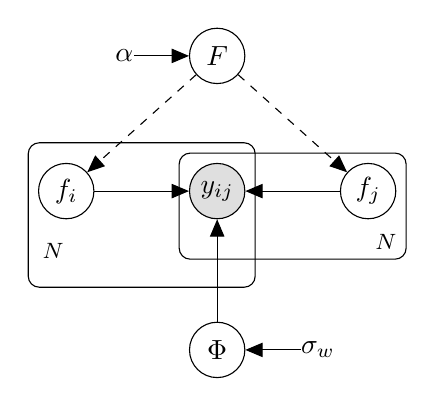
\begin{tikzpicture}
  % Define nodes
  \node[obs]                      (y) {$y_{ij}$};
  \node[latent, left=1.2cm of y] (fi) {$\mat{f}_i$};
  \node[latent, right=1.2cm of y] (fj) {$\mat{f}_j$};
  \node[latent, above= of y]    (ibp) {$\mat{F}$};;
  \node[latent, below= of y, yshift=-0.3cm]   (W) {$\mat{\Phi}$};
  \node[const, left=0.7cm of ibp]   (a) {$\alpha$};
  \node[const, right=0.7cm of W]   (sw) {$\sigma_w$};

  % Connect the nodes
  \edge {fi,fj,W} {y} ;
  \edge[dashed] {ibp} {fi,fj} ;
  \edge {sw} {W} ; 
  \edge {a} {ibp} ; 

  % Plates
  \plate {yx} {(fj)(y)} {$N$} ;
  \plate[label={[label distance=-0.6cm]195:$N$}] {} {(fi)(y)(yx.north west)(yx.south west)} {} ;
  %\plate {} {(W)} {$K\times K$};
  %\plate {} {(fi)(y)(yx.north west)(yx.south west)} {$N$} ;
\end{tikzpicture}
}
	\endminipage
	\minipage{0.4\textwidth}
	\scalebox{0.9}{
		/home/dulac/Documents/workInProgress/networkofgraphs/papers/personal/figures/draw/mmsb2.tex}
	\endminipage
	\caption{The two Graphical model for (left) the latent feature model and (right) the latent class model. The conceptual difference between the two model are the actualization of latent variables for each interaction. The latent feature model uses the same latent features vector for each node's interaction, while the latent class model draws new variables at each interactions.}
	\label{fig:ilfrm}
\end{figure}

\subsubsection{MCMC Updates for Posterior Inference}

The update for the latent features are obtained by the following Gibbs updates:
\begin{align}
& P(f_{ik} = 1 \mid F^{-ik}) = \frac{m^{-ik}}{N} \\
& P(f_{ik} = 0 \mid F^{-ik}) = 1 - \frac{m^{-ik}}{N}
\end{align}
Where $m^{-ik}$ represents the number of active features $k$ for all entities excluding entity $i$, hence $m^{-ik} = \sum_{j\neq i}f_{jk}$. 

The learning of the weight matrix $W$ is computed using a Metropolis-Hasting algorithm. Thus, we sample sequentially each weight corresponding to non-zeros features interaction.

\begin{equation}
P(\phi_{mn} \mid Y, F, \phi_{-mn}, \sigma_w) \propto P(Y \mid F, \Phi) P(\phi_{mn} \mid \sigma_w)
\end{equation}

We choose a jumping distribution in the same family of our prior on weight centered around the previous sample:

\begin{equation} \label{eq:j_w}
J(\phi_{mn}^* \mid \phi_{mn}) = \mathcal{N}(\phi_{mn}, \eta)
\end{equation}
with $\eta$ a parameter letting us controlling the acceptance ratio.

The acceptance ratio of $\phi_{mn}^*$ is thus:
\begin{equation} \label{eq:r_w}
r_{\phi_{mn}\rightarrow \phi_{mn}^*} = \frac{ P(Y \mid F, \Phi^*)P(\phi_{mn}^* \mid \sigma_w)J(\phi_{mn} \mid \phi_{mn}^*) }{ P(Y \mid F, \Phi)P(\phi_{mn} \mid \sigma_w)J(\phi_{mn}^* \mid \phi_{mn} )}
\end{equation}

\subsubsection{Properties}

In this model, the weight interaction matrix $\Phi$ are not conjugate of the likelihood. Thus it can not be integrated out into a closed form expression. As a matter of simplicity we consider this parameter as known, and omit it the following conditional distribution .

Let $F=\Theta$ and $W=\Phi$, each node $i$ has a fixed feature vector noted $F_i$ and a weighed interactions matrix $W$. In this case, the function $f_i$ is:
\begin{align}
\pr(y_{ij}=1 \mid d_i, F^{-i\bm{.}}) &= \sum_{F_i} \pr(y_{ij}=1 \mid d_i, F^{-i\bm{.}} F_i,) \pr(F_i \mid d_i, F^{-i\bm{.}}) \\
&= \sum_{F_i} \sigma(F_iWF_j^T) \frac{\pr(d_i \mid F^{-i\bm{.}}, F_i) \pr(F_i\mid F^{-i\bm{.}}) }{\pr(d_i\mid F^{-i\bm{.}})}\\
&\propto \sum_{F_i} \prod_{j' \in \V(i) \cup {j}} \sigma(F_iWF_{j'}^T)\prod_{j' \notin \V(i)} 1-\sigma(F_iWF_{j'}^T) \prod_k \frac{m_{ik}}{N}
\end{align}

The last term of equation (7.16) comes from the conditional probability of a feature $f_{ik}$ with an IBP prior and applying a chain of product rule. 

(Reste a valider le passage à la proportion !).It turns out that the $f_i$ is increasing under the assumptions that the model is \emph{strictly} (to define) homophilic. it means that if the similarity between two nodes is greater than one, with a support in $[-1, 1]$, leads to a probability greater than $\frac{1}{2}$. This justify the use of the logistic kernel. 

%The probability that a matrix $F$ is generated from the IBP is ~\cite{IBP}:
%\begin{equation}
%P(F \mid \alpha) = \frac{\alpha^{K_+}}{\prod_{i=1}^N K_1^{(i)} } \exp(-\alpha H_N) \prod_{k=1}^{K_+} \frac{(N - m_k)!(m_k - 1)!}{N!}
%\end{equation}

\subsection{Latent Class}

In the latent class model, the rows of the feature matrix $\Theta$ are Dirichlet distributed, and the weights interaction are Beta distributed : 
\begin{align}
\theta_i &\sim \mathrm{Dirichlet}(\alpha_0) \quad\text{ for }  i \in \{1, .., N\} \\
\phi_{mn} &\sim \mathrm{Beta}(\lambda) \quad\text{ for }  m,n \in \{1, .., K\}^2 
\end{align}
The observation level is defined by multinomial draws of class assignments for each nodes. The likelihood for a links depends only on the class assignments of the nodes  and for $i, j \in V$, we have:  
\begin{align}
z_{i\rightarrow j} &\sim \mathrm{Mult}(\theta_i) \\
z_{i\leftarrow j} &\sim \mathrm{Mult}(\theta_j) \\
y_{ij} &\sim \mathrm{Bern}(z_{i\rightarrow j} \Phi z_{i\leftarrow j}^\top)
\end{align}

In this special case, the mapping function $\sigma$ is the identity.

\paragraph{Altenartive Description ! (wich one we keep ?)}~\\

An alternate view, maybe more consistent with the IBP representation is to say that:
\begin{align}
Z &\sim CRF(\alpha_0, \gamma) \\
\phi_{mn} &\sim \mathrm{Beta}(\lambda) \quad\text{ for }  m,n \in \{1, .., K\}^2  \\
y_{ij} &\sim \mathrm{Bern}(\Phi_{z_{i\rightarrow j} , z_{i\leftarrow j}})
\end{align}

In the (not printed here) corresponding graphical model, the arrow between $z_{\rightarrow}$ and $Z$ are dashed as for the IBP representation. Note that $Z \in \{1,.., K\}^{N\times N \times 2}$. ~\\

@ERIC: This representation would justify to explain our interpretation for the Chinese Restaurant Franchise (CRF), because we clearly see it now...

\subsubsection{MCMC Updates for Posterior Inference}~\\

In the latent class model, the collapsed gibbs sampling approach allow us to only sample the classes couple for each observations:

\begin{equation}
\pr(z_{ji}=k, z_{ij}=k' \mid .) \propto \pr(z_{ji}=k \mid .) \pr(z_{ij}=k' \mid .) f_{(k,k')}^{-ji}(y_{ji})
\end{equation}


The class assignment updates for the node couple are:
\begin{align}
\pr(z_{i\rightarrow j} =k \mid Z^{-ij}) &\propto N_{ik}^{-ij} + \alpha_0 \\
\pr(z_{i\leftarrow j} =k \mid Z^{-ij}) &\propto N_{jk}^{-ij} + \alpha_0 
\end{align}

And the likelihood of a link given the couple $c=(k, k')$ is:
\begin{equation} \label{eq:cgs_mmsb}
f_{(k, k')}^{-ij}(y_{ij}=r) = \frac{C_{(k,k')r}^{-ij} + \lambda_r}{C_{(k,k')\bm{.}}^{-ij} + \sum_r\lambda_{r'}} 
\end{equation}

Finally $\Theta$ and $\Phi$ can be reconstructed from the count matrices with the following equations:
\begin{align}
\theta_{ik} &= \frac{N_{ik} + \alpha_0}{ N_{i\bm{.}} + K\alpha_0} \\
\phi_{rc} &= \frac{C_{cr} + \lambda_r}{ C_{c.} + \lambda_{\bm{.}}}
\end{align}

$C$ and $N$ are counts matrices and are describes in section \ref{burst_class}. We refer to the supplementary material for detail of derivations for MCMC updates. 

\subsubsection{Properties}

\label{burst_class}

In the latent class models each  dyads has two underlying  class assignments for each node of the couple. We note $Z \in N\times N\times 2$ the matrix that represents those class assignments.
We seek for the following form of the likelihood, that we marginalize over all the possible couples classes $c=(k, k')$:
\begin{equation} \label{eq:q}
\pr(y_{ij}=1 \mid Y^{-i\bm{.}}, Z^{-ij}, d_i ) = \sum_{c=(k, k')} \pr(y_{ij}=1 \mid Y^{-i\bm{.}}, d_i , c) \pr(c \mid  Z^{-ij} ) 
\end{equation}
Here note that within the sum, the left hand term is conditionally independent of $Z^{-ij}$. And the right hand term is independent of the adjacency terms $Y^{-i\bm{.}}$ since it do not belongs to the Markov blanket of $c$ random variable.

The first term is the likelihood for the links between $(i,j)$ given the class of each node (k, k'). Due to the Beta-Bernoulli conjugacy of the model, $\phi$ and $\theta$ can be marginalized out, and it simplify to: 
\begin{equation} \label{eq:qc}
\pr(y_{ij}=1 \mid Y^{-i\bm{.}}, d_i , c) = \frac{C_{c1}^{-i.} + d_{ic} + \lambda_1}{C_{c\bm{.}}^{-ij} + \lambda_0+\lambda_1} 
\end{equation}
Where $C_{c1}$ denotes the count matrix for all interactions having value 1 (link present) with the classes couple being $c=(k, k')$. Thus $C_{c1} = \sum_{i,j} \bm{1}(z_{i\rightarrow j}=k, z_{i\leftarrow j}=k', y_{ij}=1)$ and $C_{c.} = \sum_{i,j} \bm{1}(z_{i\rightarrow j}=k, z_{i\leftarrow j}=k')$\\

We recognize the likelihood form of the Gibbs update~\cite{HDP}, except that we isolate the term depending of the degree on $i$, $d_i$. Hence the term $d_{ic}$ is the element of the degree with a classes couple $c=(k,k')$ and $d_{ic} = \sum_{j' \neq j} \bm{1}(z_{i\rightarrow j'}=k, z_{i\leftarrow j'}=k', y_{ij'}=1) $.\\

The second term of equation \eqref{eq:q}, can be rewrited by noting that the classes of the couple $c$ are independent and that the term $Y^{-j\bm{.}}$ can be dropped because it is not present in the Markov blanket of the class assignment: 
\begin{equation} \label{eq:topic_assign}
\pr(c \mid  Z^{-ij} ) =  \pr(z_{i\rightarrow j}=k \mid Z^{-ij}) \pr(z_{i\leftarrow j}=k' \mid Z^{-ij})
\end{equation}

Again, the two members of the right hand equation \eqref{eq:topic_assign} are the Gibbs updates for the topic assignments of nodes for the interaction $(i,j)$. Both members reduce to simple form due to the conjugacy between the Dirichlet and Multinomial~\cite{DM} or concurrently from the Chinese Restaurant Franchise~\cite{HDP}:
\begin{align}
\pr(z_{i\rightarrow j}=k \mid Z^{-ij}) = \frac{N_{ik}^{-ij} + \alpha_k}{ N_{i.}^{-ij} + \alpha_{\bm{.}} } \\
\pr(z_{i\leftarrow j}=k' \mid Z^{-ij}) = \frac{N_{jk'}^{-ij} + \alpha_{k'}}{ N_{j\bm{.}}^{-ij} + \alpha_{\bm{.}} } 
\end{align}

Finally, one can see that the only term depending on the degree $d_i$ is isolated, and we can rewrite equation \eqref{eq:q}, with term depending only on $d_i$, $k$, $i$ and $j$:
\begin{equation}
\pr(y_{ij}=1 \mid Y^{-i\bm{.}}, Z^{-ij}, d_i ) = \sum_{c=(k, k')} A_c (B_c + d_{ic})
\end{equation}
Where $A_c$ and $B_c$ are two positive function of $c$.
\begin{align}
A_c &= \frac{N_{ik}^{-ij} + \alpha_k}{ N_{i.}^{-ij} + \alpha_{\bm{.}} } \frac{N_{jk'}^{-ij} + \alpha_{k'}}{ N_{j\bm{.}}^{-ij} + \alpha_{\bm{.}} } \frac{1}{C_{c\bm{.}}^{-ij} + \lambda_0+\lambda_1} \\
B_c &= C_{c1}^{-i.} + \lambda_1
\end{align}

As we sum over all possible couple classes, the probability to have a link will augment with the degree with the classes couple corresponding to the element of the degree with the same couple. Hence the probability to observe a link for node $i$ is strictly crescent with his degree $d_i$. 

\paragraph{Preferential Attachment}~\\

The model is bursty hence it can handle the preferential attachment at the network level.

\paragraph{Local Preferential Attachment}~\\

The Local preferential attachment is similar to the notion of burstiness but inside a community/class of the network. Assuming that we know the class of $i$ $z_{i\rightarrow j}$ to be $k$, the probability to have a link becomes: 
\begin{align}
\pr(y_{ij}=1 \mid Y^{-i\bm{.}}, d_i,z_{i\rightarrow j})  &= \sum_{k'} \pr(y_{ij}=1 \mid Y^{-i\bm{.}}, Z^{-ij}, d_i , c=(k,k')) \pr(z_{i\leftarrow j}=k' \mid Z^{-ij} ) \\
&= \sum_{k'} \frac{C_{c1}^{-i.} + d_{ic} + \lambda_1}{C_{c\bm{.}}^{-ij} + \lambda_0 + \lambda_1} \frac{N_{jk'}^{-ij} + \alpha_{k'}}{ N_{j\bm{.}}^{-ij} + \alpha_{\bm{.}} } \\
&= \sum_{k'} A'_{k'} (B'_{k'} + d_{i(k,k')})
\end{align}

Here the probability increases with the degree independently of the interactions classes. This means that burstiness is possible inside but also between communities.

\paragraph{Communities Distribution}~\\

....Need to count the table for each classes in Chinese Restaurant Franchise (CRF), to evaluate the distribution according to the hyperprior of HDP...


\subsection{Comparison of models}
class proportion vs feature vector \\
Class strength vs feature correlation/metric ? \\
HDP vs IBP \\
complextity $O((E^2K^2)$ vs $O(NK^3)$ \\
property yes/no


\section{Empirical results}

To validate our theoretical results we fitted our models on synthetic networks and track how well we can reproduce the properties of interest on a generated network.

The synthetic network has 1000 nodes and 4 communities and a density of 0.05. [See the ref of the generator for the ground true on the preferential attachment effect...]

%Our experiments evaluate the preferential attachment and the local preferential attachment on the learned communities trough respectively the distribution of degrees in the networks and inside the communities.
%\begin{figure}[h]
%	\centering
%	\includegraphics[scale=0.8]{../figures/img/prop/gen3_order_immsb_10}
%	\caption{\textbf{Adjacency matrices re-ordered according to the detected communities}}
%	\label{fig:}
%\end{figure}
%
%
%\begin{figure}[h]
%	\centering
%	
%		\minipage{0.5\textwidth}
%			\includegraphics[scale=0.4]{../figures/img/prop/gen3_com_immsb_4}
%		\endminipage
%		\minipage{0.5\textwidth}
%			\includegraphics[scale=0.4]{../figures/img/prop/gen3_com_immsb_10}
%			\endminipage
%
%	\caption{\textbf{Distribution of communities size for the class based model. The left figure correspond to number of class K=4, and the right figure correspond to K=10. The power law do not appear strongly }}
%	\label{fig:}
%\end{figure}
%
%\begin{figure}[h]
%	\centering
%	
%	\minipage{0.5\textwidth}
%	\includegraphics[scale=0.4]{../figures/img/prop/gen3_global_deg_immsb_4}
%	\endminipage
%	\minipage{0.5\textwidth}
%	\includegraphics[scale=0.4]{../figures/img/prop/gen3_global_deg_immsb_10}
%	\endminipage
%	
%	\caption{\textbf{Distribution of degree for the class based model. The left figure correspond to number of class K=4, and the right figure correspond to K=10. It appears that the model is able to capture the power law.}}
%	\label{fig:}
%\end{figure}
%
%\begin{figure}[h]
%	\centering
%	\includegraphics[scale=0.9]{../figures/img/prop/gen3_local_deg_immsb_4}
%	\caption{\textbf{Local degree distribution for 3 communities for a total of 4 classes.}}
%	\label{fig:}
%\end{figure}
%
%\begin{figure}[h]
%	\centering
%	\includegraphics[scale=0.9]{../figures/img/prop/gen3_local_deg_immsb_10}
%	\caption{\textbf{Local degree distribution for 3 communities for a total of 10 classes.}}
%	\label{fig:}
%\end{figure}
%
%
%%class based on 
%%10 classes:
%%Precision global 0.9900621488, local: 0.038679245283 , Rappel 0.0400390625
%%4 classes:
%%Precision global 0.98990976619, local: 0.0280898876404 , Rappel 0.0295275590551
%
%%IBP: K=46
%%Precision global 0.990138852919, local: 0.0488721804511 , Rappel 0.0509803921569
%
%
\clearpage

\section{Supplementary materials}

\subsection{Class based derivation}

\paragraph{Likelihood:}~\\

We mention that  the $\phi$ and $\theta$ matrix can be reconstructed with $Z$. From the model, we have the following equalities:
\begin{align}
\pr(y_{ij} \mid \phi_c) &= \phi_c^{y_{ij}}(1-\phi_c)^{1-y_{ij}} \\
\pr(\phi_c \mid \lambda) &= \frac{1}{B(\lambda_1, \lambda_0)} \phi_c^{\lambda_1-1}(1-\phi_c)^{\lambda_0 -1}
\end{align}


Derivation of equation (5.12) of the likelihood:
\begin{align}
&\pr(y_{ij} \mid Y^{-ij}, c) \propto \pr(y_{ij}, Y^{-ij}, c) \\
&= \int_{\phi_c} \pr(y_{ij} \mid \phi_c) \pr(\phi_c \mid \lambda) \prod_{i'j' \neq ij}\pr(y_{i'j'} \mid \phi_c) d\phi_c \\
&\propto \int_{\phi_c} \phi_c^{y_{ij} + C_{c1}^{-ji} + \lambda_1-1}(1-\phi_c)^{ 1-y_{ij} + C_{c0}^{-ji} + \lambda_0 -1} d\phi_c \\
&\propto \frac{\Gamma(y_{ij} + C_{c1}^{-ji} + \lambda_1) \Gamma( 1-y_{ij} + C_{c0}^{-ji} + \lambda_0) }{\Gamma(  1+ C_{c\bm{.}}^{-ji} + \lambda_0 + \lambda_1)}
\end{align}

Considering the case where $y_{ij} =1$, we have :
\begin{equation}
\pr(y_{ij}=1 \mid \phi_c) = \frac{C_{c1}^{-ji} + \lambda_1}{C_{c\bm{.}}^{-ji} + \lambda_0 + \lambda_1}
\end{equation}


\paragraph{Class Assignment:}~\\

We have from the model the following equalities:
\begin{align}
\pr(\theta_i \mid \alpha) &= \frac{\Gamma(\sum_l \alpha)}{\prod_l \Gamma(\alpha)} \prod_l \theta_{il}^{\alpha-1} \\
\pr(z_{i\rightarrow j} &= k \mid \theta_i) = \theta_{ik}
\end{align}

Derivation of equation (5.14) of class assignment:
\begin{align}
&\pr(z_{i\rightarrow j}=k \mid Z^{-ij}) = \pr(z_{i\rightarrow j}=k \mid \{z_{i\rightarrow j_0}\}_{j_0\neq j},\{z_{i\leftarrow j_0}\}_{j_0= 1}^n )\\
&\propto \pr(z_{i\rightarrow j}= k,\{z_{i\rightarrow j_0}\}_{j_0\neq j},\{z_{i\leftarrow j_0}\}_{j_0= 1}^n ) \\
&= \int_{\theta_i} \pr(\theta_i \mid \alpha) \pr(z_{i\rightarrow j}=k \mid \theta_i) \prod_{j_0\neq j} \pr(z_{i\rightarrow j_0} \mid \theta_i) \prod_{j_0 =  1}^n  \pr(z_{i\leftarrow j_0} \mid \theta_i)  d\theta_i \\
&=\int_{\theta_i} \frac{\Gamma(\sum_l \alpha)}{\prod_l \Gamma(\alpha)}\theta_{ik}^{N_{ik}^{-ji}+1} \prod_{l\neq k} \theta_{il}^{N_{il}^{-ij} +\alpha-1} d\theta_i \\
&\propto \frac{\Gamma(\alpha + N_{ik}^{-ji}+1)\prod_{l\neq k} \Gamma(\alpha + N_{il}^{-ij})}{\Gamma(\sum_l( \alpha + N_{il}^{-ji}) +1)} \\
&\propto \alpha + N_{ik}^{-ji}
\end{align}

Finally the equality is maintain by the marginalization constant:
\begin{equation}
\pr(z_{i\rightarrow j}=k \mid Z^{-ij}) =\frac{ N_{ik}^{-ji} + \alpha}{ N_{i\bm{.}}^{-ji} + K\alpha }
\end{equation}

\subsection{Burstiness for degrees Distribution}
\label{burst_proof}

From the definition of the burstiness, we have for a random variable $d$:
\begin{equation}
	\pr(d \geq n'+1 \mid d \geq n') > \pr(d \geq n+1 \mid d \geq n) \quad \{\forall (n,n') \mid  n' > n \}
\end{equation}

We now consider the degree $d_i$ for a node $i$ of a network. We can rewrite the burstiness in the discrete case:
\begin{equation}
\pr(d_i = n'+1 \mid d_i = n') > \pr(d_i = n+1 \mid d_i = n), \quad \{\forall (n,n') \mid  n' > n \}
\end{equation}
\hspace{0.35\textwidth} Q. is it equivalent to: $\pr(d_i)' > 0$ ?\\

Let's suppose that the model $\mathcal{M} = \{\Theta, \Phi\}$ has converged to some local optima. Do new predictions will respect the burstiness property ? To answer this question we need to evaluate the predictive distribution and we assume that the model parameters for all data except for node $i$ is knows. Hence, we denote this knowledge as $\mathcal{M}^{-i}$ whose condition the degree distribution. We omit reference to it in the following. Additionally we write $\pr(d_i)$ accounting for $\pr(d_i=n)$:
\begin{align}
    \pr(d_i=n+1 \mid d_i) &= \sum_{\mathcal{M}_i} \pr(d_i=n+1 \mid d_i, \mathcal{M}_i) \pr(\mathcal{M}_i \mid d_i)
\end{align}
The likelihood of the degree can now be written using the conditional independence. Note that we omit reference to the model parameters $\mathcal{M}$:
\begin{align}
    \pr(d_i=n+1 \mid d_i) &= \sum_{j \notin \mathcal{V}(i)} \pr(y_{ij} = 1 \mid d_i) \prod_{j'\notin \mathcal{V}(i), j' \neq j} \pr(y_{ij'}=0 \mid d_i) \\
    &=  \sum_{j \notin \mathcal{V}(i)} (1 - \pr(y_{ij} = 0 \mid d_i) ) \prod_{j'\notin \mathcal{V}(i), j' \neq j} \pr(y_{ij'}=0 \mid d_i) \\
    &= ...
\end{align}
Where $\mathcal{V}(i)$ represent all vertex connected to $i$ and $| \mathcal{V}(i) | = d_i$.\\



\bibliographystyle{unsrt}
\bibliography{../bibd}

\end{document}
